\documentclass[12pt]{extarticle}
\title{Continuity in Metric Spaces and Topologies}
\author{Avinash Iyer, Occidental College}
\date{}
\usepackage[shortlabels]{enumitem}


%paper setup
\usepackage{geometry}
\geometry{letterpaper, portrait, margin=1in}
\usepackage{fancyhdr}
\usepackage{cmbright}
%symbols
\usepackage{amsmath}
\usepackage{amssymb}
\usepackage{amsthm}
\usepackage{mathtools}
\usepackage[hidelinks]{hyperref}
\usepackage{gensymb}
\usepackage{multirow,array}

\newtheorem*{remark}{Remark}
\usepackage[T1]{fontenc}
\usepackage[utf8]{inputenc}

%chemistry stuff
%\usepackage[version=4]{mhchem}
%\usepackage{chemfig}

%plotting
\usepackage{pgfplots}
\usepackage{tikz}
\tikzset{middleweight/.style={pos = 0.5, fill=white}}
\tikzset{weight/.style={pos = 0.5, fill = white}}
\tikzset{lateweight/.style={pos = 0.75, fill = white}}
\tikzset{earlyweight/.style={pos = 0.25, fill=white}}

%\usepackage{natbib}

%graphics stuff
\usepackage{graphicx}
\usepackage[backend=bibtex,style=numeric,sorting=none]{biblatex} %Imports biblatex package
\addbibresource{sample.bib} %Import the bibliography file
%code stuff
%when using minted, make sure to add the -shell-escape flag
%you can use lstlisting if you don't want to use minted
%\usepackage{minted}
%\usemintedstyle{pastie}
%\newminted[javacode]{java}{frame=lines,framesep=2mm,linenos=true,fontsize=\footnotesize,tabsize=3,autogobble,}
%\newminted[cppcode]{cpp}{frame=lines,framesep=2mm,linenos=true,fontsize=\footnotesize,tabsize=3,autogobble,}

%\usepackage{listings}
%\usepackage{color}
%\definecolor{dkgreen}{rgb}{0,0.6,0}
%\definecolor{gray}{rgb}{0.5,0.5,0.5}
%\definecolor{mauve}{rgb}{0.58,0,0.82}
%
%\lstset{frame=tb,
%	language=Java,
%	aboveskip=3mm,
%	belowskip=3mm,
%	showstringspaces=false,
%	columns=flexible,
%	basicstyle={\small\ttfamily},
%	numbers=none,
%	numberstyle=\tiny\color{gray},
%	keywordstyle=\color{blue},
%	commentstyle=\color{dkgreen},
%	stringstyle=\color{mauve},
%	breaklines=true,
%	breakatwhitespace=true,
%	tabsize=3
%}
% text + color boxes
\usepackage[most]{tcolorbox}
\tcbuselibrary{breakable}
\newtcolorbox{problem}[1]{colback = white, title = {#1}, breakable}
\newtcolorbox{solution}{colback = white, colframe = black!75!white, title = Solution, breakable}
%including PDFs
%\usepackage{pdfpages}
\setlength{\parindent}{0pt}
\usepackage{cancel}
\newcommand{\card}{\text{card}}
\newcommand{\ran}{\text{ran}}
\newcommand{\N}{\mathbb{N}}
\newcommand{\Q}{\mathbb{Q}}
\newcommand{\Z}{\mathbb{Z}}
\newcommand{\R}{\mathbb{R}}
\usepackage{setspace}
\begin{document}
\doublespacing
  \begin{center}
    \large \sc Homeomorphism between the Open Ball Topology on $\R^2$ and the Open Rectangle Topology on $\R^2$
  \end{center}
  \begin{center}
    Avinash Iyer\\
    Occidental College
  \end{center}
  Word Count: 1191.
  \section*{Abstract}%
  In this paper, I introduce the concept of metric spaces (including the definition of distance metrics, open sets, and continuity), topologies on sets, and homeomorphisms. With this knowledge, we can prove that the Open Rectangle Topology, where we view $\R^2$ as a union of Cartesian products of open intervals, and the Open Ball Topology, where we view $\R^2$ as an open disc, are equivalent ways of viewing $\R^2$, or that they're homeomorphic.
  \section*{Motivation}%
  In 200-level math, we got a sense of understanding as to some of the properties of the real number line --- such as distance between two elements, $|x-y|$, for example. However, things become much more complicated and fascinating when we implement more rigor into the definition of ``distance,'' and even more so as we enter higher dimensions.\\

  For example we might ask what the ``shape'' of the plane, $\R^2$ is. On first look, it seems obvious --- the plane $\R^2$ is just the Cartesian product of the real line with itself --- but as mentioned before, we need to understand what the properties of the real line are, and how those translate into $\R^2$. Similarly, we might view $\R^2$ as polar in nature --- its shape similar to that of a disc. As we approach the edge of this edgeless disc, the radius in $\R^2$ approaches infinity.\\

  \begin{center}
    The plane as a ``square:''\\
    \vspace{12pt}
    \begin{tikzpicture}
      \draw[dashed](0,0) -- (0,3) -- (3,3) -- (3,0) -- cycle;
    \end{tikzpicture}
    \vspace{12pt}\\
    The plane as a ``disc:''\\
    \vspace{12pt}
    \begin{tikzpicture}
      \draw[dashed] (0,0) circle(1.5);
    \end{tikzpicture}
  \end{center}
  All of these and more must be rigorously defined --- so let's get started.
  \section*{Metric Spaces, Open Sets, and Continuity}%
  Consider a set $X$, with $a,b\in X$. It's often useful to consider the idea of a distance between $a$ and $b$, $d(a,b)$. This distance function must map every pair of points to some positive number.
  \begin{align*}
    d: X\times X \rightarrow \R^+
  \end{align*}
  Additionally, it has to have the following properties:
  \begin{itemize}
    \item Zero distance property: $d(a,a) = 0$ and if $d(a,b) = 0$, then $a = b$.
    \item Commutativity: $d(a,b) = d(b,a)$.
    \item Triangle Inequality: $d(x,z) = d(x,y) + d(y,z)$.
  \end{itemize}
  This defines a \textbf{distance metric} on $X$. For instance, for $x,y\in\R^n$, we define the \textbf{Euclidean metric} as follows:
  \begin{align*}
    d(x,y) = \left(\sum_{i=1}^{n}(x_i-y_i)^2\right)^{1/2}
  \end{align*}
  In $\R^1 = \R$, this is equivalent to $|x-y|$.\\

  In $\R^n$ with the Euclidean metric, we define the \textbf{open ball} of radius $\varepsilon > 0$ about the point $x$ as follows:
  \begin{align*}
    V_{\varepsilon} &= \left\{p \mid d(x,p) < \varepsilon\right\}
  \end{align*}
  In $\R$, this equivalent to the open interval $(x-\varepsilon,x+\varepsilon)$.\\

  In $A\subseteq X$, if $\forall~x\in A,~\exists~\varepsilon > 0$ such that $V_{\varepsilon}(x)\subseteq A$, then $A$ is an \textbf{open set}. If $A = \emptyset$ or $A = X$, then $A$ is open. Every open ball is an open set.
  \begin{description}
    \item[Proposition:] Let $A$ and $B$ be open sets in a metric space $X$. Then, $A\cap B$ and $A\cup B$ are open sets in $X$.
    \item[Proof:] Let $a\in A$ and $b\in B$. Then, $\exists~\varepsilon_a>0$ such that $V_{\varepsilon_a}(a)\subseteq A$, meaning that $V_{\varepsilon_a}(a)\subseteq A\cup B$, and similarly for $b$ and $\varepsilon_b$.\\

    If $A = \emptyset$, then $A\cap B = \emptyset$, meaning $A\cap B$ is open. Otherwise, suppose $A\cap B \neq \emptyset$. Let $x\in A\cap B$, meaning $x\in A$ and $x\in B$. So, $\exists~\varepsilon_1>0$ such that $V_{\varepsilon_1}(x)\in A$.\\

    Specifically, define $\varepsilon_1$ to be the maximum such value. Similarly, $\exists~\varepsilon_2 > 0$ such that $V_{\varepsilon_2}(x)\in B$, where $\varepsilon_2$ is the maximum such value. Let $\varepsilon = \min\{\varepsilon_1,\varepsilon_2\}$ Then, $V_{\varepsilon} \subseteq V_{\varepsilon_1}$ and $V_{\varepsilon} \subseteq V_{\varepsilon_2}$, meaning $V_{\varepsilon} \subseteq A$ and $V_{\varepsilon}\subseteq B$, so $V_{\varepsilon} \subseteq A\cap B$.
  \end{description}
  Consider a function in a metric space $f: X\rightarrow Y$. Just as with functions in the real numbers, we can consider the continuity of $f$.\supercite{lay} Specifically, $f$ is continuous if $\forall~x_1,x_2\in X$
  \begin{align*}
    \left(\forall~\varepsilon > 0\right)\left(\exists~\delta > 0\right)~\text{such that}~d(x_1,x_2) < \delta \Rightarrow d(f(x_1),f(x_2))<\varepsilon.
  \end{align*}
  Alternatively, this can be phrased as
  \begin{align*}
    \left(\forall~\varepsilon > 0\right)\left(\exists~\delta > 0\right)~\text{such that}~\forall~a,~a\in V_{\delta}(x) \Rightarrow f(a)\in V_{\varepsilon}(f(x)).
  \end{align*}
  \begin{description}
    \item[Proposition:] If $f:X\rightarrow Y$ is continuous, then $\forall~x\in X,~f(V_{\delta}(x)) \subseteq V_{\varepsilon}(f(x))$ for some $\varepsilon,\delta > 0$.
    \item[Proof:] Let $\varepsilon > 0$ and $f: X\rightarrow Y$ be continuous. For $x,a\in X$, define $\delta > 0$ such that $d(x,a) < \delta \Rightarrow d(f(x),f(a)) < \varepsilon$, which exists by definition of continuity.\\

      Then, $a\in V_{\delta}(x)$, meaning $f(a)\in f(V_{\delta}(x))$, and $f(a)\in V_{\varepsilon}(f(x))$ as defined earlier. Therefore, $f(V_{\delta}(x))\subseteq V_{\varepsilon}(f(x))$.
  \end{description}
  Using this result, we can prove an important fact of continuity.
  \begin{description}
    \item[Proposition:] $f: X\rightarrow Y$ is continuous if and only if the preimage of every open set in $Y$ is open in $X$.
    \item[Proof:]
      \begin{description}
        \item[$(\Rightarrow)$] Let $f$ be a continuous function. If $B\subseteq Y$ is open, then $\forall~y\in B,~\exists~\varepsilon > 0$ such that $V_{\varepsilon}(y) \subseteq B$. Since $x\in Y$, $\exists~x\in X$ such that $f(x) = y$, meaning $V_{\varepsilon}(f(x)) \subseteq B$.\\

          By our previous result, we know $\exists~\delta > 0$ such that $f(V_{\delta}(x))\subseteq V_{\varepsilon}(f(x))\subseteq B$, meaning $V_{\delta}(x) \subseteq f^{-1}(B)$. Therefore, $f^{-1}(B)$ is open.
        \item[$(\Leftarrow)$] Let $f: X \rightarrow Y$ be defined such that for every open $B\subseteq Y$, $f^{-1}(B)$ is open in $X$. Let $B$ be open in $Y$, and $x\in f^{-1}(B)$, meaning $f(x)\in B$.\\

          Since $B$ is open in $X$ and $f^{-1}(B)$ is open in $Y$, we know $\exists~\varepsilon > 0$ such that $V_{\varepsilon}(f(x))\subseteq B$.\\

          By definition, every open ball is an open set, meaning $f^{-1}(V_{\varepsilon}(f(x)))$ is open in $X$.Similarly, since $x\in f^{-1}(B)$, $\exists~\delta > 0$ such that $V_{\delta}(x)\subseteq f^{-1}(V_{\varepsilon}(f(x)))$.\\

          Therefore, $\forall~\varepsilon > 0$, we have a suitable $\delta$ defined as above such that $\forall~a$ such that $a\in V_{\delta}(x)$, $f(a)\in V_{\varepsilon}(f(x))$.
      \end{description}
  \end{description}
  \section*{Topology with Metric Spaces}%
  We can generalize the concept of open sets and continuity using the properties above to sets without a metric. For this purpose, on a set $L$, we define a \textbf{topology} on $L$, $ \mathcal{T}(L) $, to be a set of open sets defined as follows:
  \begin{itemize}
    \item $L, \emptyset \in \mathcal{T}(L)$
    \item if $A,B\in \mathcal{T}(L)$, then $A\cap B$ and $A\cup B\in \mathcal{T}(L)$
  \end{itemize}
  For a metric space $X$, the topology \textbf{induced} by the metric is the set of open sets in $X$. Similar to continuity in a metric space, we define continuity on a function between topological spaces by the following:
  \begin{quote}
    The function $f: X\rightarrow Y$ between topological spaces $X$ and $Y$ is continuous if and only if the preimage of every open set in $Y$ is open in $X$.
  \end{quote}
  Recall that a given topological space $X$ has two properties:
  \begin{itemize}
    \item Elements: $X = \{x_1,x_2,\dots\}$
    \item Open Sets: $A_1,A_2,A_3,\dots \subseteq X$
  \end{itemize}
  Consider two topological spaces, $X$ and $Y$. If we want to consider an idea that $X$ and $Y$ are ``equal,'' we must find a correspondence such that both the open sets and the elements correspond to each other one to one.\\

  Let $f: X\rightarrow Y$ be defined as follows:
  \begin{itemize}
    \item $f$ is a bijection.
    \item $f$ is continuous.
    \item $f^{-1}$ is continuous.
  \end{itemize}
  Then we know that each open set in $X$ corresponds to one, and only one, open set in $Y$, and each element in $X$ corresponds to one, and only one, element in $Y$. The function $f$ is a \textbf{homeomorphism}, and if such an $f$ exists, then $X$ is \textbf{homeomorphic} to $Y$.
  \section*{Two Topologies on $\R^2$}%
  Consider two topologies, $ \mathcal{T}_R $ and $ \mathcal{T}_V $, defining open sets in $\R^2$.
  \begin{itemize}
    \item The ``Open Rectangle Topology'' on $\R^2$ is defined by a union of Cartesian products of open intervals.
      \begin{align*}
        \bigcup_{i=1}^{n}(a_i,b_i)\times(c_i,d_i) \in \mathcal{T}_R
      \end{align*}
    \item The ``Open Ball Topology'' on $\R^2$ is defined by a union of open balls.
      \begin{align*}
        \bigcup_{i=1}^{n}V_{\varepsilon_i}(x) \in \mathcal{T}_V
      \end{align*}
  \end{itemize}
  We can view these two topologies as akin to the aforementioned view of $\R^2$ as a Cartesian product, and $\R^2$ as polar in nature. With the open rectangle topology, we view a given point in the plane as being within an interval of $\R$ in the $x$ coordinate and a given interval of $\R$ in the $y$ coordinate. Meanwhile, with the open ball topology, we view a given point in the plane as being some distance $d$ away from a different point in space. Each point of the open ball topology is in some ``circle'' surrounding said point, while each point of the open rectangle topology is in some square or rectangle surrounding the point.\\

  At first glance these two views of $\R^2$ look nothing alike --- a rectangle is clearly a quite different shape than that of a circle. However, the question posed at the beginning --- what the ``shape'' of $\R^2$ is --- has a distinct answer when we see it through this lens. Namely, the open rectangle and the open ball are \textit{the same} --- that is, they are homeomorphic.
  \begin{description}
    \item[Proposition:]$ \mathcal{T}_V(\R^2) $ and $ \mathcal{T}_R(\R^2) $ are homeomorphic.
    \item[Proof:] Let $f: \R^2 \rightarrow \R^2$ be defined as $f(x) = x$. We will show that every open set in $\mathcal{T}_R$ is open in $\mathcal{T}_V$, and vice versa.\\

      Consider an open set $A\in\mathcal{T}_R$ --- we will show that this open set is open in $\mathcal{T}_V$.\\

      Let $(a,b)\times(c,d)\subseteq A$ be an open rectangle, and $x = (x_a,y_a)\in (a,b)\times(c,d)$. We can always find $\varepsilon = \min\left\{|x_a-a|,|x_a-b|,|y_a-c|,|y_a-d|\right\}$ such that $V_{\varepsilon}(x) \subseteq (a,b)\times (c,d)$. Therefore, this open rectangle is open in $\mathcal{T}_V$, and since every open set in $\mathcal{T}_R$ is a union of open rectangles, and each open rectangle is open in $\mathcal{T}_V$, the union of these open rectangles is open in $\mathcal{T}_V$.
      \begin{center}
        Open Rectangle to Open Ball Continuity:\\
        \vspace{12pt}
        \begin{tikzpicture}
          \draw[black!50!white,dashed] (0,-5) -- (0,7) -- (5,7) -- (5,-5) -- cycle;
          \filldraw (3,4) circle (2pt);
          \draw (3,4) --node[middleweight,anchor = south]{$\varepsilon$} (5,4);
          \node[anchor = east] at (3,4) {$a$};
          \draw[dashed] (3,4) circle(2);
        \end{tikzpicture}
      \end{center}
      Consider an open set $B\in\mathcal{T}_V$. Let $V_{\varepsilon}(x)\subseteq B$ be an open ball centered at $x = (x_x,x_y)$. Let $a=(a_x,a_y)\in V_{\varepsilon}(x)$ be a point in $V_{\varepsilon}(x)$.\\

      Since $V_{\varepsilon}(x)$ is open, $\exists~\delta$ such that $V_{\delta}(a)\subseteq V_{\varepsilon}(x)$. Define the open rectangle to be $A = (a_x-\delta/\sqrt{2},a_x+\delta/\sqrt{2})\times(a_y-\delta/\sqrt{2},a_y + \delta/\sqrt{2})$ Then, this open rectangle is a subset of $V_{\delta}(a)\subseteq V_{\varepsilon}(x)$, meaning $V_{\varepsilon}(x)$ is open in $\mathcal{T}_R$. Since $\mathcal{T}_V$ is a union of open balls, and the union of these open sets is open, the union of open balls is open in $\mathcal{T}_R$.\\
        \begin{center}
          Open Ball to Open Rectangle Continuity:\\
          \vspace{12pt}
          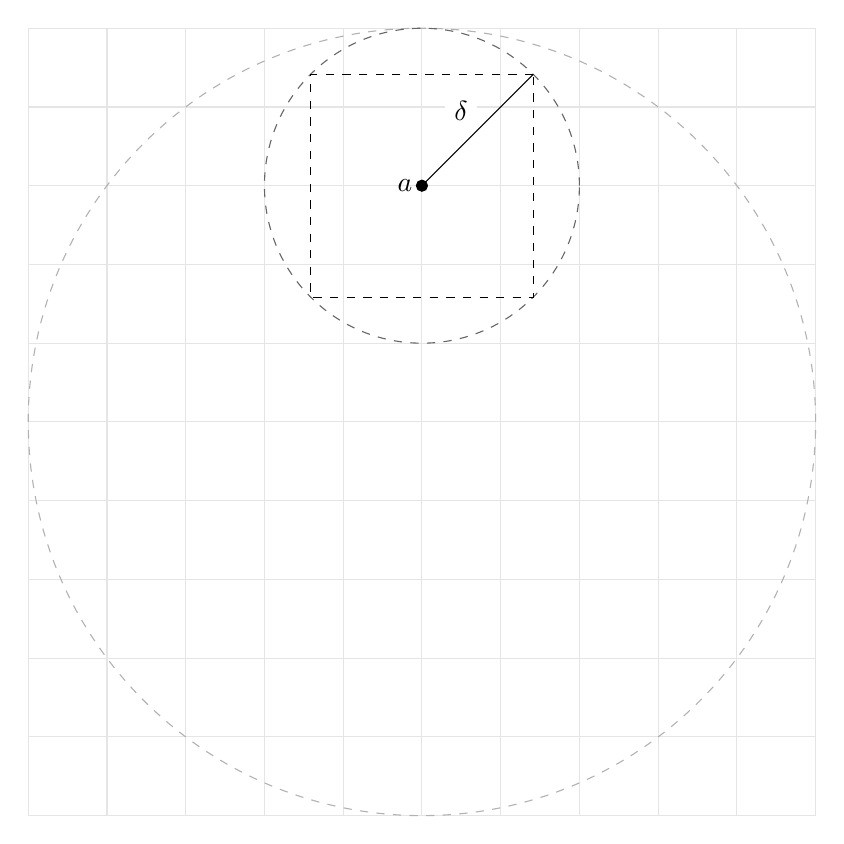
\begin{tikzpicture}
            \draw[color = black!10!white] (-5,-5) grid (5,5);
            \draw[color=black!30!white,dashed] (0,0) circle(5);
            \filldraw (0,3) circle(2pt);
            \node[anchor = east] at (0,3){$a$};
            \draw[color=black!60!white,dashed] (0,3) circle (2);
            \draw[dashed] (1.414,4.414) -- (-1.414,4.414) -- (-1.414,1.585) -- (1.414,1.585) -- cycle;
            \draw (0,3) --node[middleweight,anchor=south east]{$\delta$} (1.414,4.414);
          \end{tikzpicture}
        \end{center}
  \end{description}
  \section*{Acknowledgments}%
  I would like to thank professor Ramin Naimi, whose Math 362 class was indispensable in developing the background necessary to show this result.
  \printbibliography
\end{document}
